\documentclass[tikz,dvipsnames]{standalone}
\usepackage{tikz-feynman}

\begin{document}

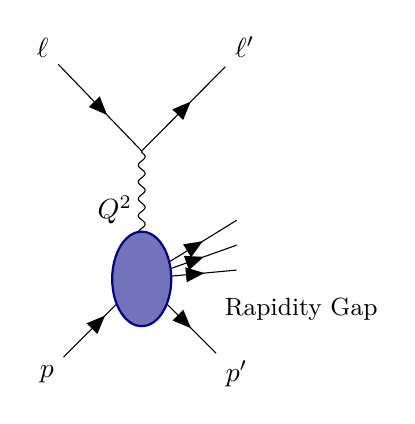
\begin{tikzpicture}[scale=1.5]
    \begin{feynman}        
            \vertex (a);
            \vertex (i1) [above left= of a]{\(\ell\)};
            \vertex (i2) [above right= of a] {\(\ell'\)};
            \vertex (b)[below= of a] {};
    
            \vertex (f1)[below left= 4.85em of b] {\(p\)};
            \vertex (f2)[below right= 4.85em of b] {\(p'\)};
            \vertex (f3)[above=5.55em of f2] ;
            \vertex (f4)[above=4.65em of f2] ;
            \vertex (f5)[above=3.75em of f2] ;
            \vertex (f6)[above right=3.3em of f2] {\small{Rapidity Gap}} ;
            
            \diagram*{
            (i1)  -- [fermion] (a) -- [fermion] (i2) ,
            (a) -- [photon, edge label'=\(Q^{2}\)] (b) ,
            (f1) -- [fermion]  (b)   -- [fermion] (f2) ,
            (b) -- [fermion] (f3),
            (b) -- [fermion] (f4),
            (b) -- [fermion] (f5), 
            };
         
    \end{feynman}
    \fill[NavyBlue!55] (b) ellipse (0.25 and 0.4);
    \draw[NavyBlue, thick] (b) ellipse (0.25 and 0.4);
    \end{tikzpicture}
    
\end{document}